\section{Middleboxes: Design \& Implementation}
\label{sec:mbs}

In Table~\ref{tbl:mbreqs}, we introduced the set of middleboxes typically supported by outsourcing approaches and divided them in to Header, HTTP, and DPI middleboxes. 
We now revisit these middleboxes individually and discuss how they operate over the encrypted data.

\eat{
\begin{figure}[t]
  \centering
  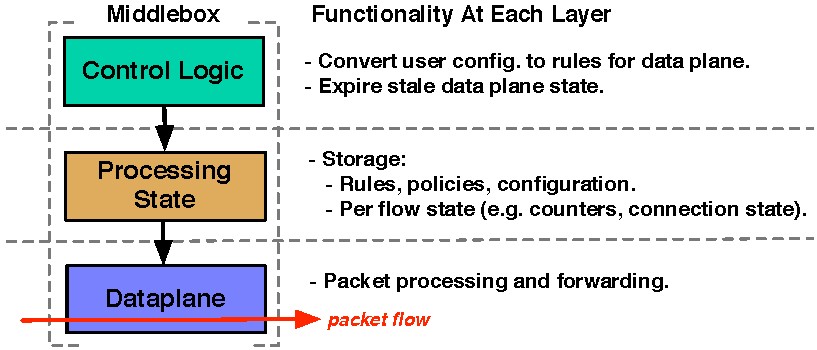
\includegraphics[width=3in]{fig/mbarch}
  \caption[]{\label{fig:mbarch} Typical middlebox software components. For most middleboxes, packet processing operations in the dataplane remain unmodified by \sys. \justine{Cut? Unnecessary?}}
\end{figure}
}

\subsection{Header Middleboxes}
Middleboxes which operate on IP and transport headers only include firewalls, NATs, and L4 load balancers.
Firewalls are read-only, but NATs and L4 load balancers may rewrite IP addresses or port values. 
For header middleboxes, per-packet operations remain unchanged for both read and write operations.

For read operations, the firewall receives a set of encrypted rules from the gateway and compares them directly against the encrypted packets just as normal traffic. Because RangeMatch supports $\leq$ and $\geq$, the firewall may use any of the standard classification algorithms~\cite{packet_classif}.

For write operations, the middleboxes assign values from an address pool; it receives these encrypted pool values from the gateway during the rule generation phase.
These encrypted rules are marked with a special suffix reserved for rewritten values.
When the gateway receives a packet with such a rewritten value, it restores the plaintext value from the pool rather than decrypting the value from the options header.

\subsection{DPI Middleboxes}
We modify middleboxes which perform DPI operations as described by BlindBox~\cite{blindbox}; unlike header middleboxes these devices must be rewritten in per-packet behavior to support encrypted traffic.
The middleboxes search through the encrypted extension channel -- not the packet payloads themselves -- and block the connection if a blacklisted term is observed in the extension.

\subsection{HTTP Middleboxes}
Parental filters and L7 Load Balancers read the HTTP URI from the options header. 
If the parental filter observes a blacklisted URI, it drops the connection.
The L7 load balancer uses the URI to rewrite the IP header, and operates exactly like a NAT or L4 LB, except that it uses the URI to select which destination address to assign new connections.

The proxy required the most modification of any middlebox \sys supports; nonetheless, our proxy achieves good performance as we will discuss in \S\ref{sec:eval}.
The proxy  caches HTTP static content (e.g., images) in order to improve client-side performance. 
When a client opens a new HTTP connection, a typical proxy will capture the client's SYN packet and open a new connection to the client, as if the proxy were the web server. The proxy then opens a second connection in the background to the original web server, as if it were the client. 
When a client sends a request for new content, if the content is in the proxy's cache, the proxy will serve it from there. Otherwise, the proxy will forward this request to the web server and cache the new content. 

The proxy has a map of encrypted file path to encrypted file content. When the proxy receives a packet, the proxy extracts the encrypted URI from the options header and looks it up in the cache {\em as if it were not encrypted}. The use of deterministic encryption enables the proxy to use a fast search data structure/index, such as a hash map, unchanged. We have two cases: there is a hit or a miss. For hit, the proxy assembles a packet header for reverse traffic and attaches to it the encrypted file content from the cache. Even without being able to encrypt IP addresses or ports, the proxy can create the header by reversing the encrypted information in the original header.
For a miss, the proxy forwards the request to the web server. When receiving the response, the proxy caches it to serve future requests.



